\chapter{Differential Algebraic Equations}

von num gew dgl niochtsteife steife und dae

\subsection{Abstract Problem}
\begin{equation}
	\label{Abstract_DAE}
	F(t, y(t), y'(t)) = 0 \qquad \forall t \in I
\end{equation}

with $F:\mathbb{R} \times \mathbb{R}^N \times \mathbb{R}^N \to \mathbb{R}^N$ sufficiently smooth. We will focus on linear time invaraiant systems of the form

\begin{displaymath}
	E u'(t) = A u(t) + f(t).
\end{displaymath}

With $E, A \in \mathbb{R}^{n \times n}$. If $E$ is regular, then this system is just an ordinary differential equation, thus we assume $E$ to be singular to obtain a ``true'' DAE. 

In the following chapters we will discuss important analytical properties of this such sytems. We will discuss the solvability and the index of these systems.

\subsection{Types of DAEs}

\begin{itemize}
	\item \textbf{Linear systems with constant coeffiecients} \newline
	are systems of the form 
	\begin{equation}
		\label{DAE-const-coeff}
		A y'(t) + B y(t) = f(t)
	\end{equation}
	with $A,B \in \mathbb{R}^{n \times n}$, $A$ singular and $f(t)$ a function.
	\item \textbf{linear time dependent systems}
	\begin{displaymath}
		A(t) y'(t) + B(t) y(t) = f(t)
	\end{displaymath}
	with $A(t),B(t),f(t)$ functions.
	\item  \textbf{structured (non-linear) systems} \newline
	are semi-explicit systems of the form
	\begin{displaymath}
		y'(t) = f(t, y(t), z(t)),
		0 = g(t,y(t),z(t))
	\end{displaymath}
	with $f$ and $g$ functions.
\end{itemize}

For our analysis of electrical networks we will focus on linear systems with constant coefficients. (where do the other systems arrise? what are they about?)

\subsubsection{Weierstraß-Kronecker Normalform}
kapitel aus buch seite 399 num gew dgl steif, kapitel 13.2.2

To determine the solvability of a linear system with constant coefficients \ref{DAE-const-coeff} we first need to introduce a Normalform for the system, the \emph{Weierstraß-Kronecker Normalform}. This Normalform is dependant on the family $\{A,B\} := \{ \mu A+B|\mu \in \mathbb{R} \}$, which is called the  \emph{matrix pencil} of the DAE.

\begin{definition}
	The matrix pencil $\{ A,B\}$ is called \emph{regular} if there exists some $c \in \mathbb{R}$, such that $(cA+B)$ is regular ($det(cA+B) \neq 0$), otherwise it is called singular.
\end{definition}

\begin{theorem}[Jordan Normalform]
	For every matrix $Q \in \mathbb{R^{n \times n}}$ there exists a regular matrix $T \in \mathbb{C}^{n \times n}$, such that
	\begin{displaymath}
		T^{-1}QT = J = diag(J_1, ..., J_r) \quad \text{with} \quad J_i = 
		\left(
		\begin{matrix}
			\lambda_i & 1 & & 0 \\
			0 & \lambda_i & \ddots & \vdots \\
			& \ddots & \ddots & 1 \\
			0 & \hdots & 0 & \lambda_i
		\end{matrix}
		\right)
		\in \mathbb{C}^{m_i \times m_i}
	\end{displaymath} 
	and $n = m_1 + ... + m_r$.
\end{theorem}
quote that from somewhere.

translate that:

The matrix $J$ is called Jordan Normalform of $Q$, the $J_i$ are called Jordan Blocks, where $\lambda_i$ are the eigenvalues of $Q$. The matrix $J$ is uniquely determined by $Q$ except for the arrangement of the diagonal blocks. If $Q$ posesses only real eigenvalues, then $T$ can also be choosen from the reals. \newline
A transformation from $A$ and $B$ in \ref{DAE-const-coeff} enables a seperation into differential and algebraic variables.	

aus buch seite 401
\begin{theorem}
	\label{Kronecker-Normalform}
	Let $\{ A,B \}$ be a regular matrix pencil. There exist $P,Q \in \mathbb{C}^{n \times n}$ such that
	\begin{displaymath}
		PAQ = 
		\left(
		\begin{matrix}
			I_d & 0 \\
			0 & N 
		\end{matrix}
		\right), \quad
		PBQ = 
		\left(
		\begin{matrix}
			R & 0 \\
			0 & I_{n-d}
		\end{matrix}
		\right)
	\end{displaymath}
	where
	\begin{displaymath}
		N = diag(N_1, ..., N_r) \quad \text{with} \quad N_i = 
		\left(
		\begin{matrix}
			0 & 1 & & 0\\
			& \ddots &\ddots & \\
			& & & 0 & 1 \\
			0 & & & 0
		\end{matrix}
		\right)
		\in \mathbb{R}^{n_i \times n_i}
	\end{displaymath}
	and R has Jordan Normalform.
\end{theorem}
\begin{proof}
	Becuase $\{A,B\}$ is a regular matrix pencil, there exists $c \in \mathbb{R}$ such that $(cA+B)$ is regular. Set
	\begin{displaymath}
		\hat{A} := (cA+B)^{-1}A, \quad \hat{B} := (cA+B)^{-1}B.
	\end{displaymath}
	Considering 
	\begin{displaymath}
		(cA+B)^{-1}(cA+B) = I \implies (cA+B)^{-1}B+c(cA+B)^{-1}A = I ,
	\end{displaymath}
	we get that
	\begin{displaymath}
		\hat{B} = I-c \hat{A} .
	\end{displaymath}
	Let $J_ {\hat{A}}$ be the Jordan Normalform of $\hat{A}$, this means that there exists a regular matrix $T_1$ such that
	\begin{displaymath}
		T_1^{-1}AT_1 = J_{\hat{A}} =
		\left(
		\begin{matrix}
			W & 0 \\
			0 & \tilde{N} 
		\end{matrix}
		\right) .
	\end{displaymath}
	The matrix $W$ contains the Jordanblocks with Eigenvalues which are nonzero, the matrix $\tilde{N}$ contains the Jordan blocks with Eigenvalues equal to zero, thus $\tilde{N}$ is \emph{nilpotent}.
	The Jordan Normalform $J_{\hat{B}}$ of $\hat{B}$ is given by
	\begin{displaymath}
		T_1^{-1} \hat{B} T_1 = J_{\hat{B}} = 
		\left(
		\begin{matrix}
			I-cW & 0 \\
			0 & I-c\tilde{N}
		\end{matrix}
		\right) .
	\end{displaymath}
	The following two transformations will allow us to get the desired structure.
	First we will transform $J_{\hat{A}}$ with
	\begin{displaymath}
		T_2 :=
		\left(
		\begin{matrix}
			W & 0 \\
			0 & I-c\tilde{N}
		\end{matrix}
		\right)
	\end{displaymath}
	in
	\begin{displaymath}
		T_2^{-1}J_{\hat{A}} = 
		\left(
		\begin{matrix}
			I & 0 \\
			0 & (I-c\tilde{N})^{-1}\tilde{N}
		\end{matrix}
		\right)
	\end{displaymath}
	and $J_{\hat{B}}$ in
	\begin{displaymath}
		T_2^{-1}J_{\hat{B}} =
		\left(
		\begin{matrix}
			W^{-1}-cI & 0 \\
			0 & I
		\end{matrix}
		\right) .
	\end{displaymath}
	Let now $R$ be the Jordan Normalform of $(W^{-1}-cI)$ and $N$ be the Normalform of $(I-c\tilde{N})^{-1}\tilde{N}$, this means
	\begin{displaymath}
		T_W^{-1}(W^{-1}-cI)T_W = R \quad \text{and} \quad T_{\tilde{N}}^{-1}(I-c\tilde{N})^{-1}\tilde{N}T_{\tilde{N}} = N
	\end{displaymath}
	Considering
	
	\begin{figure}[H]
		\centering
		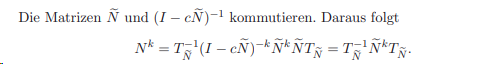
\includegraphics[width=0.7\linewidth]{screenshot001}
		\caption{fig 1, i dont get why}
		\label{fig:screenshot001}
	\end{figure}
	
	
	The nilpotent matrix $N$ thus has the nilpotency index $k$. A transformation with
	\begin{displaymath}
		T_3 := 
		\left(
		\begin{matrix}
			T_W & 0 \\
			0 & T_{\tilde{N}}
		\end{matrix}
		\right)
	\end{displaymath}
	transforms $T_2^{-1}J_{\hat{A}}$ into the Jordan Normalform
	\begin{displaymath}
		J_{\tilde{A}} := T_3^{-1}T_2^{-1}J_{\hat{A}}T_3 = T_3^{-1}T_2^{-1}T_1^{-1}\hat{A}T_1T_3 = 
		\left(
		\begin{matrix}
			I & 0 \\
			0 & N
		\end{matrix}
		\right)
	\end{displaymath}
	and $T_2^{-1}J_{\hat{B}}$ into
	\begin{displaymath}
		J_{\tilde{B}} := T_3^{-1}T_2^{-1}J_{\hat{B}}T_3 = T_3^{-1}T_2^{-1}T_1^{-1}\hat{B}T_1T_3 = 
		\left(
		\begin{matrix}
			R & 0 \\
			0 & I
		\end{matrix}
		\right) .
	\end{displaymath}
	Now set
	\begin{displaymath}
		P:= T_3^{-1}T_2^{-1}T_1^{-1}(cA+B)^{-1} \quad \text{and} \quad Q = T_1T_3
	\end{displaymath}
	to get the statement.
\end{proof}

\begin{definition}
	The nilpotency index $k$ from the Weierstraß-Kronecker Normalform of a matrix pencil $\{A,B\}$ with $A$ singular is called the \emph{Kronecker-Index} of $\{A,B\}$. We write $ind\{A,B\}$. For $A$ regular we set $ind\{A,B\} = 0$.
\end{definition}

next lemma needs quotation, it is lemma 13.2.1

\begin{lemma}
	The Kronecker-Index $ind\{A,B\}$ is independant of the choice of the matrices $P$ and $Q$.
\end{lemma}

\begin{figure}
	\centering
	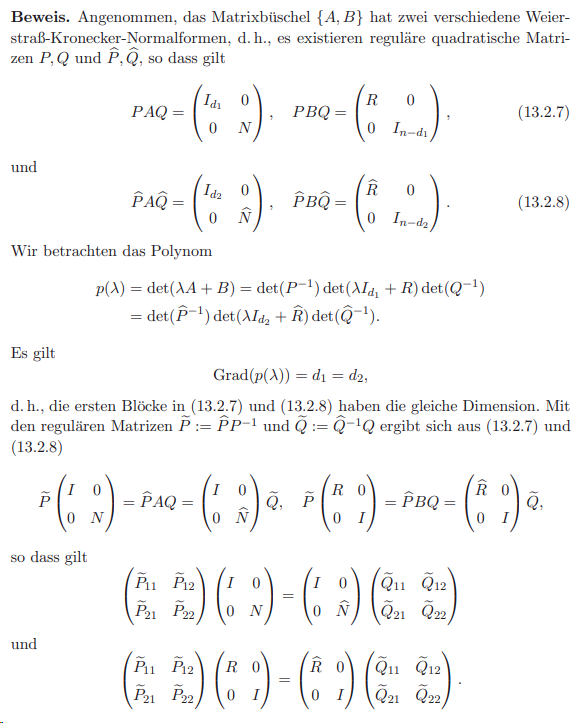
\includegraphics[width=0.7\linewidth]{screenshot003}
	\caption{}
	\label{fig:screenshot003}
\end{figure}

\begin{figure}
	\centering
	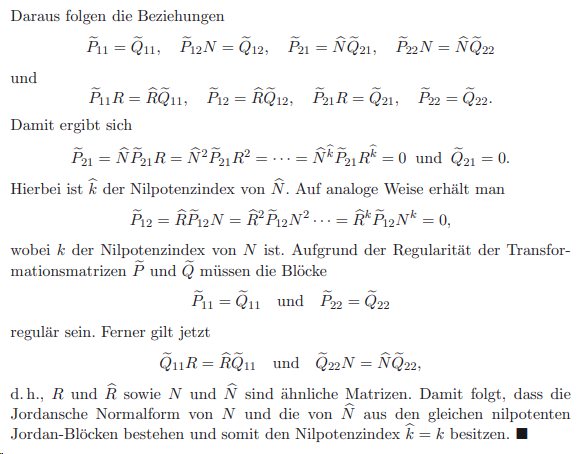
\includegraphics[width=0.7\linewidth]{screenshot004}
	\caption{}
	\label{fig:screenshot004}
\end{figure}


Lemma 13.2.2 maybe

Using the findings above we are able to Transform the initial DAE \ref{DAE-const-coeff} using the matrix $P$ from \ref{Kronecker-Normalform}. By multiplying $P$ from the left we obtain

\begin{displaymath}
	P A y'(t) + P B y(t) = P f(t) .
\end{displaymath}

Setting

\begin{displaymath}
	y = Q
	\left(
	\begin{matrix}
		u \\
		v
	\end{matrix}  
	\right) 
	, \quad
	Pf(t) = 
	\left(
	\begin{matrix}
		s(t) \\
		q(t)
	\end{matrix}
	\right)
	\quad \text{with} \quad
	u,s \in \mathbb{R}^d ,
\end{displaymath}

we get a system of the form

\begin{equation}
	\label{transformed-DAE-const-coeff}
	\begin{aligned}
		u'(t) + Ru(t) &= s(t) \\
		Nv'(t) + v(t) &= q(t)
	\end{aligned}
\end{equation}

The first equation is an ordinary differential equation of first order and posesses a unique solution $u(t)$ in $[t_0,t_l]$ for any starting values $u_0 \in \mathbb{R}^d$. Additionally setting $q(t) \in C^{k-1}([t_0,t_l])$ then differentiating the second equation in \ref{transformed-DAE-const-coeff} gives (\textbf{whyyyyyyy??????})

\begin{displaymath}
	\begin{aligned}
		v(t) &= q(t) - Nv'(t) = q(t) - N(q(t)-Nv'(t))' = q-Nq'+N^2v'' \\
		&= q-Nq'+N^2(q-Nv')'' = q-Nq'+N^2q''-N^3v''' \\
		&\vdots \\
		&= q-Nq'+...+(-1)^{k-1}N^{k-1}q^{(k-1)}+(-1) \underbrace{N^kv^{(k)}}_{=0}
	\end{aligned}
\end{displaymath}
\begin{equation}
	\label{solution-to-transformed-DAE-const-coeff-part2}
	= \sum_{i=0}^{k-1} (-1)^iN^iq^{(i)}(t) 
\end{equation}
where $k$ is the nilpotency index of $N$. This expression gives an explicit solution for $v(t)$ in $[t_0,t_l]$ with $v(t) \in \mathbb{R}^{d-1}$. It shows the depencdency of the solution and its derivatives. The higher the Kronecker index $k$ gets, the more differentiations of $q(t)$ have to be performed.

The Kronecker index $k$ shows, that $k$ differentiations are required to receive an ordinary differential equation.

\subsection{Index of a Differential Algebraic Equation}

The Index of a DAE gives us insight about it's numerical properties and in general about the solvability. In general, the higher the index, the harder it is, to solve the system. 

We will consider two types of index concepts, the differentiation index and the perturbation index.

\begin{definition}[differentiation index]
	Consider the differential algebraic equation \ref{Abstract_DAE} to be uniquely locally solvable and $F$ suffieciently smooth differentiable. For a given $m \in \mathbb{N}$ consider
	\begin{displaymath}
		\begin{aligned}
			F(t,y,y') &= 0, \\
			\diff{F(t,y,y')}{t} &= 0, \\
			&\vdotswithin{=} \\
			\diff[m]{F(t,y,y')}{t} &= 0.
		\end{aligned}
	\end{displaymath}
	The smallest natural number $m$ for which the above System results in an explicit system of the form
	\begin{displaymath}
		y' = \phi(t,y)
	\end{displaymath}
	from which $y$ can be determined is called \textbf{differentiation index}.
\end{definition}

In the previous chapter we have already discussed, that for a DAE with constant coefficients \ref{DAE-const-coeff} and a regular matrix pencil $\{A,B\}$  we need $k = ind\{A,B\}$ differentiations to receive an ordinary differential equation. This means that the Kronecker index $k$ is equal to the differentiation index in the case of a DAE with constant coefficients.

\begin{definition}[perturbation index]
	Let $y(t)$ be the exact solution to \ref{Abstract_DAE}. This problem has the \textbf{perturbation index} $k \in \mathbb{N}$ along $y(t), t_0 \leq t \leq T$ if for all  $\tilde{y}(t)$ with $F(t, \tilde{y}, \tilde{y}') = \delta(t)$ the inequality
	\begin{displaymath}
		||y(t)-\tilde{y}(t)|| \leq C \left(||y(t_0)-\tilde{y}(t_0)||+\sum_{j=0}^{k}\max_{t_0 \leq \xi \leq T} \left\rVert 		\int_{t_0}^{\xi}\diff[j]{\delta}{\tau}(\tau)d \tau \right\rVert \right)
	\end{displaymath}
	for the smallest number $k$.
\end{definition}	

for lin const nilpot ind  = ind + proof

\begin{figure}[H]
	\centering
	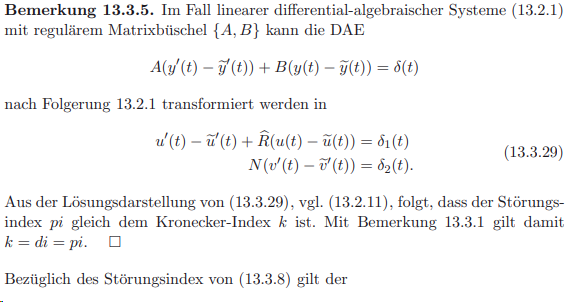
\includegraphics[width=0.7\linewidth]{screenshot005}
	\caption{}
	\label{fig:screenshot005}
\end{figure}